\section{1174017 - Muh. Rifky Prananda}
\subsection{Teori}
\begin{enumerate}
	\item Sejarah dan Perkembangan
	\hfill\break
	Kecerdasan Buatan atau dalam bahasa Inggris sering disebut Kecerdasan Buatan yang sering juga disebut sebagai AI, dalam 10 tahun terakhir orang tidak terlalu mengetahuinya dan masih bercanda di antara orang-orang. Pengembangan awal AI dimulai pada tahun 1952-1969 yang dimulai dengan keberhasilan Newwell dan temannya Simon menggunakan program yang disebut General Problem Solver. Program ini dibangun untuk tujuan memecahkan masalah secara manusiawi. Pada 1966-1974, perkembangan kecerdasan buatan mulai melambat. Ada 3 faktor utama yang menyebabkannya terjadi:
	\begin{itemize}
		\item Banyak subjek pada program AI yang bermunculan hanya mengandung sedikit atau bahkan sama sekali tidak  mengandung sama sekali pengetahuan (knowledge).
		\item Kecerdasan buatan harus bisa menyelesaikan banyak masalah.
		\item Untuk menghasilkan perilkau intelijensia ada beberapa batasan pada struktur yang bisa digunakan.
	\end{itemize}
	Definisi kecerdasan buatan itu sendiri adalah suatu system teknologi yang didalamnya ditambahakan kecerdasan oleh manusia, kecerdasan buatan diatur dan dikembangkan dalam konteks ilmiah, dan bentukan dari kecerdasan entitas ilmiah yang ada.
	\item Definisi
	\hfill\break
	Supervised learning, klasifikasi, regresi, unsupervised learning, dataset, trainingset dan testingset.
	\begin{itemize}
		\item Supervised Learning
		\hfill\break
		Supervised Learning merupakan sebuah tipe learning yang mempunyai variable input dan variable output, tipe ini juga menggunakan satu algoritma atau lebih dari satu algoritma yang digunakan untuk mempelajari fungsi  pemetaan dari input ke output.
		\item Klasifikasi
		\hfill\break
		Klasifikasi adalah pengelompokan data di mana data yang digunakan memiliki label atau kelas target. Sehingga algoritma untuk menyelesaikan masalah klasifikasi dikategorikan ke dalam pembelajaran terbimbing.
		\item Regresi
		\hfill\break
		regressi metode analisis statistik yang digunakan untuk dapat melihat efek antara dua atau lebih variabel. Hubungan variabel dalam pertanyaan adalah fungsional yang diwujudkan dalam bentuk model matematika. Dalam analisis regresi, variabel dibagi menjadi dua jenis, yaitu variabel respons atau yang biasa disebut variabel dependen dan variabel independen atau dikenal sebagai variabel independen. Ada beberapa jenis analisis regresi, yaitu regresi sederhana yang mencakup linear sederhana dan regresi non-linear sederhana dan regresi berganda yang mencakup banyak linier atau non-linear berganda. Analisis regresi digunakan dalam pembelajaran mesin pembelajaran dengan metode pembelajaran terawasi.
		\item Unsupervised learning 
		\hfill\break
		unsupervised learning jenis pembelajaran di mana kita hanya memiliki data input (input data) tetapi tidak ada variabel output yang terkait. Tujuan dari pembelajaran tanpa pengawasan adalah untuk memodelkan struktur dasar atau distribusi data dengan tujuan mempelajari data lebih lanjut, dengan kata lain, itu adalah fungsi simpulan yang menggambarkan atau menjelaskan data.
		\item Data set
		\hfill\break
		Data set objek yang merepresentasikan data dan relasinya di memory. Strukturnya mirip dengan data di database. Dataset berisi koleksi dari datatable dan datarelation.
		\item Training Set
		\hfill\break
		Training set adalah bagian dari dataset yang di latih untuk membuat prediksi atau menjalankan fungsi dari algoritma ML lain sesuai dengan masing-masing. Memberikan instruksi melalui algoritma sehingga mesin yang di praktikkan dapat menemukan korelasinya sendiri.
		\item Testing Set
		\hfill\break
		testing set adalah bagian dari dataset yang kami uji untuk melihat akurasinya, atau dengan kata lain untuk melihat kinerjanya.
	\end{itemize}
\end{enumerate}
\subsection{Praktek}
\begin{enumerate}
	\item Instalasi Library scikit dari ianaconda, mencoba kompilasi dan uji coba ambil contoh kode dan lihat variabel explorer
	\hfill\break
	\begin{figure}[H]
		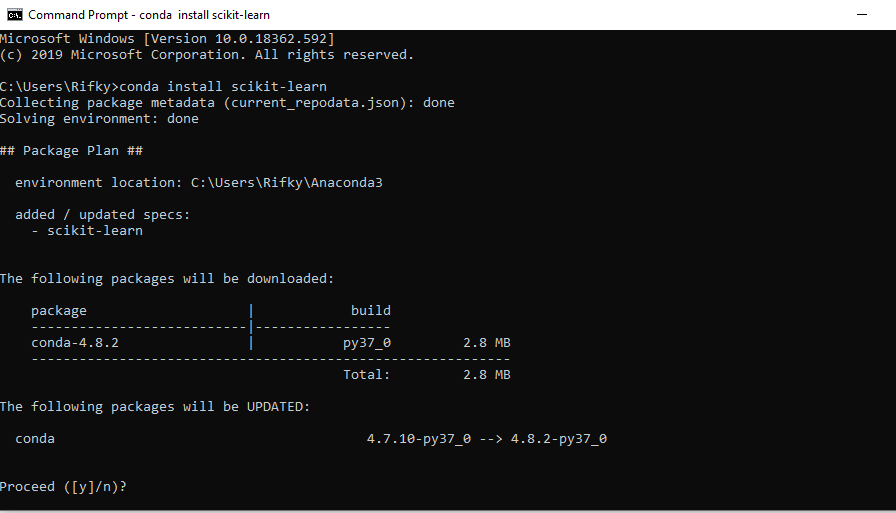
\includegraphics[width=4cm]{figures/1174017/1/instalasi.png}
		\centering
		\caption{Instalasi Package Scikit Learn}
	\end{figure}
	\begin{figure}[H]
		\includegraphics[width=4cm]{figures/1174017/1/Variabel.png}
		\centering
		\caption{Isi Variabel Explorer}
	\end{figure}
	\item Mencoba loading an example dataset
	\hfill\break
	\lstinputlisting[firstline=7, lastline=11]{src/1174017/1/1174017.py}
	\item Mencoba Learning dan predicting
	\hfill\break
	\lstinputlisting[firstline=13, lastline=22]{src/1174017/1/1174017.py}
	\item Mencoba Model Persistence
	\hfill\break
	\lstinputlisting[firstline=25, lastline=34]{src/1174017/1/1174017.py}
	\item Mencoba Conventions
	\hfill\break
	\lstinputlisting[firstline=37, lastline=48]{src/1174017/1/1174017.py}
\end{enumerate}
\subsection{Penanganan Error}
\begin{enumerate}
	\item ScreenShoot Error
	\begin{figure}[H]
		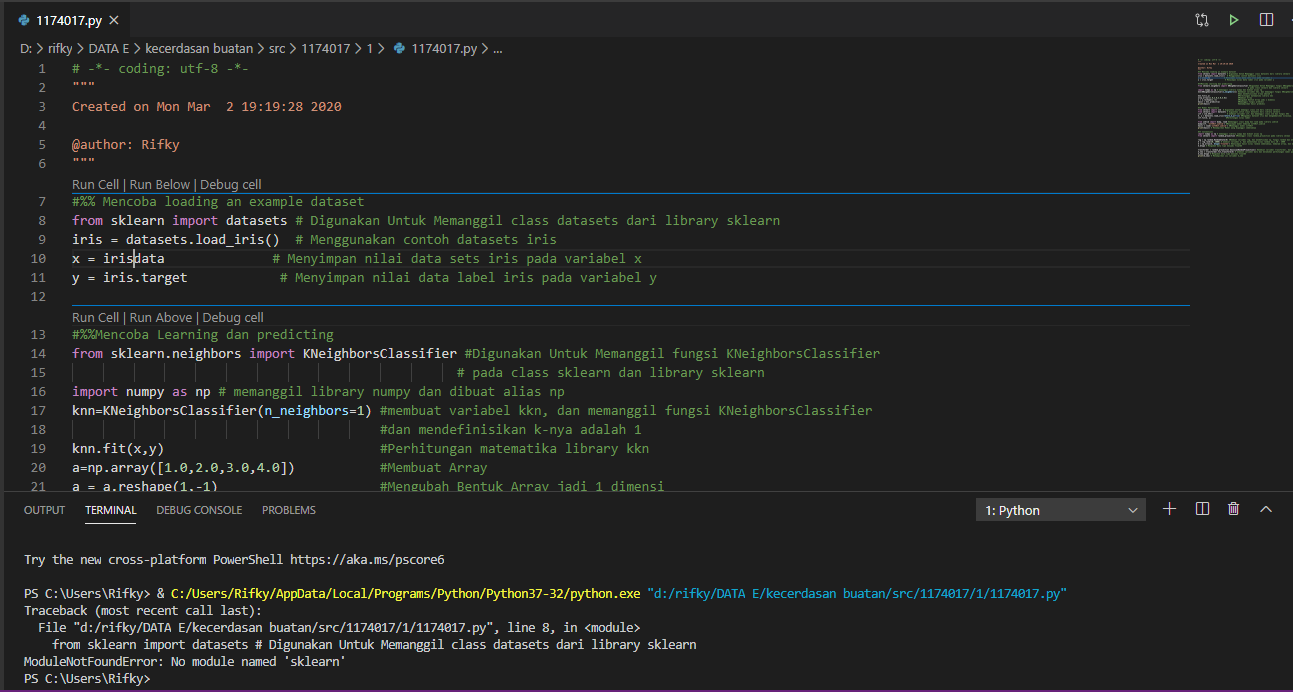
\includegraphics[width=4cm]{figures/1174017/error/1_import.png}
		\centering
		\caption{Import Error}
	\end{figure}
	\begin{figure}[H]
		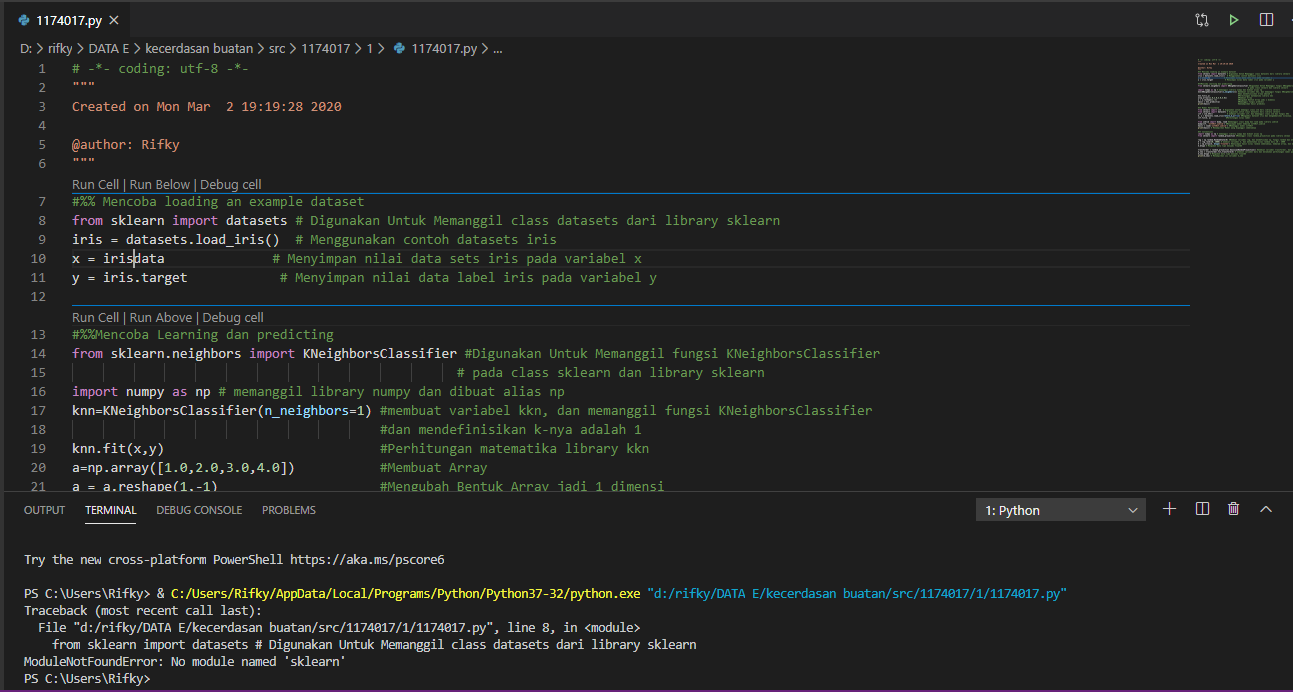
\includegraphics[width=4cm]{figures/1174017/error/1_value.png}
		\centering
		\caption{Value Error}
	\end{figure}
	\item Tuliskan Kode Error dan Jenis Error
	\begin{itemize}
		\item Import Error
		\item Value Error
	\end{itemize}
	\item Cara Penangan Error
	\begin{itemize}
		\item Import Error
		\hfill\break
		Dengan Menginstall Library Yang Tidak Ditemukan
		\item Value Error
		\hfill\break
		Mengubah Bentuk Arraynya, Menjadi 1 Dimensi
	\end{itemize}
\end{enumerate}
\subsection{Bukti Tidak Plagiat}
\begin{figure}[H]
	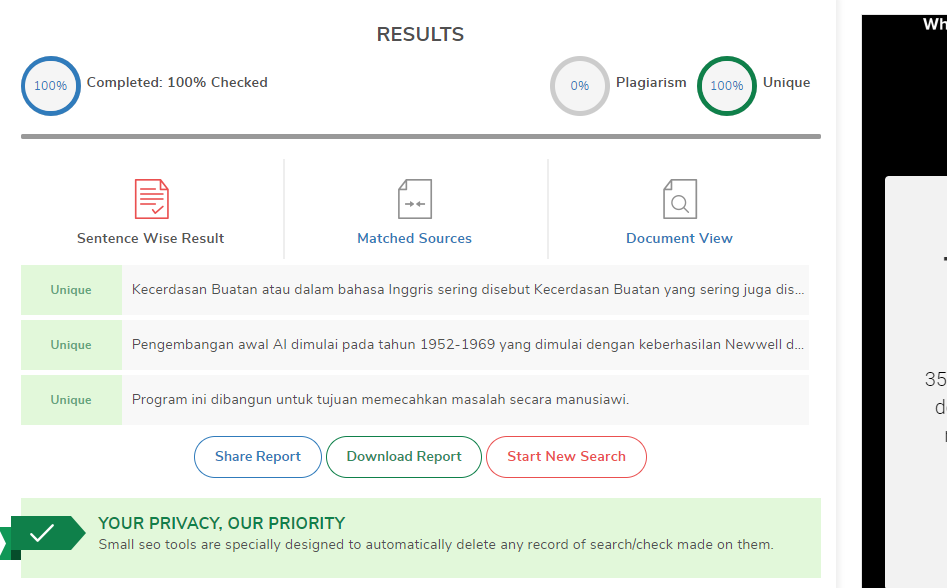
\includegraphics[width=4cm]{figures/1174017/bukti/1.png}
	\centering
	\caption{Bukti Tidak Melakukan Plagiat Chapter 1}
\end{figure}